%% -*- latex -*-
\documentclass[a4paper]{tufte-handout}

\usepackage[british]{babel}
\usepackage{booktabs}
\usepackage{tikz}
\usepackage{tikz-timing}
\usepackage{minted}
\usepackage{graphicx}
\usepackage{natbib}
\usepackage{siunitx}
\usepackage[theorems,skins]{tcolorbox}
\tcbset{enhanced}
\newtcbtheorem{exercise}{Exercise}{drop fuzzy shadow}{ex}
\newtcbtheorem{question}{Question}{drop fuzzy shadow}{q}

\title{LPC4088 Timer Interrupts\\\small{CM0506 Small Embedded Systems}}
\author{Dr Alun Moon}
\date{Seminar 5}
\definecolor{code}{wave}{602}
%\definecolor{cmd}{wave}{528}
\definecolor{cmd}{named}{SkyBlue}

\begin{document}
\maketitle

\newthought{Here the module begins to separate from EN0572.}
The programming structure will make extensive use of interrupts to
handle events, along-side a \emph{main-loop} handling polling and time
consuming actions.

Note: \emph{No Operating System}

\clearpage
\section{Timers and Interrupts}
\newthought{Attention can now be turned to the Timers and
  corresponding interrupts.}  These can be used to trigger periodic
events in some fashion.  The LPC4088 has four timers, each of which
operate in the same way.  See pages
\pageref{sec:timer-behavior}--\pageref{sec:timer-behavior-end} for
details of how the processor's internals work.

\subsection{Timer Init}
The code used for initialising a  timer.  Most of these have the
required values, some are changed for different uses.  
\begin{minted}[frame=leftline,framerule=1mm,rulecolor=\color{code}]{C}
LPC_SC->PCONP |= (1UL << 1);
LPC_TIM0->TCR = 0;
LPC_TIM0->PR = 59999;
LPC_TIM0->CTCR = 0;
LPC_TIM0->MR0 = period_ms - 1;
LPC_TIM0->MCR = 0x03UL;
timer0UserDefinedHandler = handler;
LPC_TIM0->IR = 0x3F;
NVIC_EnableIRQ(TIMER0_IRQn);
LPC_TIM0->TCR |= (1UL << 0);
\end{minted}
A line-by-line discussion of the values used follows.  Table 539 on
page 691 of the User manual \citep{lpc4088} is a good summary of the
register functions.

\begin{minted}[frame=leftline,framerule=1mm,rulecolor=\color{code}]{C}
LPC_SC->PCONP |= (1UL << 1);
\end{minted}
The PCONP register controls power to the peripheral devices.  Bit 1 is
the power supply for Timer-0 (see \citep[Table 14, pg.30]{lpc4088})

\begin{minted}[frame=leftline,framerule=1mm,rulecolor=\color{code}]{C}
LPC_TIM0->TCR = 0;
\end{minted}
The Timer control register \citep[24.6.2]{lpc4088} switches the timer
on and off.  Disabling the timer while configuring it is important for
correct behaviour to occur.

\begin{minted}[frame=leftline,framerule=1mm,rulecolor=\color{code}]{C}
LPC_TIM0->PR = 59999;
\end{minted}
The prescale register \citep[24.6.4]{lpc4088} controls the rate at
which the Timer ticks.  The Timer counts one tick for each (PR+1)
ticks of the peripheral clock (\SI{60}{\mega\hertz}).  Setting the
value to 59999 makes the timer count for every 60000 ticks of the
Peripheral clock, or $60000\times\SI{60}{\mega\hertz} =
\SI{1}{\milli\second}$. 

\begin{minted}[frame=leftline,framerule=1mm,rulecolor=\color{code}]{C}
LPC_TIM0->CTCR = 0;
\end{minted}
The count-control-register \citep[24.6.11]{lpc4088} selects whether the
system is used as a clock (Peripheral Clock) or a counter.  By setting
it to 0 we are using the device as a counter.

\begin{minted}[frame=leftline,framerule=1mm,rulecolor=\color{code}]{C}
LPC_TIM0->MR0 = period_ms - 1;
\end{minted}
Match Register 0, is one of the 4 Match Registers for the timer
\citep[24.6.7]{lpc4088}.  An interrupt occurs every (MR+1) ticks of
the Timer.  Since we have make the clock tick once every
\SI{1}{\milli\second}, we just need the period in \si{\milli\second}
minus 1.

\begin{minted}[frame=leftline,framerule=1mm,rulecolor=\color{code}]{C}
LPC_TIM0->MCR = 0x03UL;
\end{minted}
The Match Control Register \citep[24.6.6]{lpc4088} determines what
actions occur, when the timer count (CR) equals one of the match
registers (MR\textit{n}).  Setting bit 0 causes an interrupt to be
generated, setting bit 1 causes a timer reset.

\begin{minted}[frame=leftline,framerule=1mm,rulecolor=\color{code}]{C}
timer0UserDefinedHandler = handler;
\end{minted}
This saves a user defined function for use in the ISR.

\begin{minted}[frame=leftline,framerule=1mm,rulecolor=\color{code}]{C}
LPC_TIM0->IR = 0x3F;
\end{minted}
The Interrupt Register \citep[24.6.1]{lpc4088} indicates which
interrupt has occurred.  Writing 1s to this register resets the
corresponding interrupt.

\begin{minted}[frame=leftline,framerule=1mm,rulecolor=\color{code}]{C}
NVIC_EnableIRQ(TIMER0_IRQn);
\end{minted}
Enables the timer-0 interrupts (see \citep[Chapter 5]{lpc4088}.

\begin{minted}[frame=leftline,framerule=1mm,rulecolor=\color{code}]{C}
LPC_TIM0->TCR |= (1UL << 0);
\end{minted}
The Timer control register \citep[24.6.2]{lpc4088} switches the timer
on and off.  Setting bit 0 enables the timer,  \emph{note} bit 1 is
kept clear.

\subsection{ISR}
The Interrupt-Service-Routine is show below.
\begin{minted}[frame=leftline,framerule=1mm,rulecolor=\color{code}]{C}
void TIMER0_IRQHandler(void) {
	timer0UserDefinedHandler();
	LPC_TIM0->IR |= (1UL << 0);
}
\end{minted}
The first line calls the function stored from the Timer init function.
The second line writes a 1 to bit 0 resetting the interrupt.  If this
bit is \emph{not} reset, then no further interrupts can occur.

\paragraph{The Timing Diagram for timer interrupts} is shown in table
\ref{tab:timing}.  It is shown for a hypothetical case with the
prescale register set to 2 (PR=2) and the match register 1 (MR{\it n}=1). 
\begin{table*}
  \begin{tabular}{rl}
    Peripheral clock & \texttiming{26{C}} \\
    Prescale counter & \texttiming{D{}4{2D{0}2D{1}2D{2}}D} \\
    Timer counter    & \texttiming{D{}2{6D{0}6D{1}}D} \\
    Interrupt        & \texttiming{L2{G12L}GL} \\
    ISR              & \texttiming{L2{2H10L}HH}\\
  \end{tabular}
\caption{Timing diagram}
\label{tab:timing}
\end{table*}

\section{Simple Flashing}
Example 1.2 just flashes one LED in a simple fashion.
\begin{minted}[frame=leftline,framerule=1mm,rulecolor=\color{cmd}]{bash}
$ git clone https://github.com/dr-alun-moon/timers
$ cd timers
$ git checkout ex.1.2
\end{minted}
\begin{exercise}{Add a second LED}{two-led}
  Add code to use a second timer (Timer-1) to flash a second LED at a
  different rate.

  If you use a multiple of the rate on Timer-0, it is easier to check
  the operation is as you'd expect.
\begin{tcolorbox}[colframe=red!50!black,title=Solution]
A solution is in Git 
\begin{minted}[frame=leftline,framerule=1mm,rulecolor=\color{cmd}]{bash}
$ git checkout s.1.2
\end{minted}
\end{tcolorbox}\end{exercise}

A possible timing diagram is shown in table \ref{tab:twoleds},
assuming the LED state is toggled in each ISR.
\begin{table}
  \begin{tabular}{rl}\toprule
    Interrupt 0      & \texttiming{L2{G12L}GL} \\
    LED              & \texttiming{L{12H12L}H} \\ \midrule
    Interrupt 1      & \texttiming{L4{G6L}GL} \\
    LED              & \texttiming{L2{6H6L}H} \\ \bottomrule
  \end{tabular}
\caption{Timing diagram for two LEDs}
\label{tab:twoleds}
\end{table}

\clearpage
\section{Multiple Interrupts}
\newthought{Each timer can have up to 4 interrupts.}  Generated by
each of the 4 match registers.  One will have to be configured to
reset the timer, which gives the timer period (time between
interrupts).  The other three will have values less than the timer
period to cause interrupts at (up to) 3 points within the timer
period.  The Match Control Register \citep[24.6.6]{lpc4088}, has bits
to enable the interrupts for each of the match registers.  
\paragraph{These share the same interrupt routine.}  The interrupt
handler will have to interrogate the Interript Register (IR)
\citep[24.6.1]{lpc4088} to determine which match register caused the
interrupt.

\subsection{Setting up MR1}
\newthought{To set up an interrupt on MR1.}  We need to write a value
into it, and set the appropriate flag in the MCR.  The value needs to
be a fraction of the value in MR0, or else the interrupt will never
occur.  A fraction can be passed to \texttt{timer0Init} as a
\texttt{float}, and then used to multiply MR0.  Bit 3 in the match
control register needs to be set to enable the interrupt.  Finally the
interrupt handler needs to test the interrupt register (IR) to see
which match register caused the interrupt.

\marginnote{A 20\% duty cycle means that the LED is on for the first
  20\% of the flashing period.}
\begin{exercise}{LED1 on a 20\% duty cycle}{duty1}
The code in branch ex.1.3 has been modified to set up timer-0 to flash
one LED on a 20\% duty cycle.
\begin{minted}[frame=leftline,framerule=1mm,rulecolor=\color{cmd}]{bash}
$ git clone https://github.com/dr-alun-moon/timers
$ cd timers
$ git checkout ex.1.3
\end{minted}
Examine \path{main.c}, \path{timer.c}, and \path{timer.h} to check how
the changes have been made.

\begin{enumerate}
\item Add similar changes to enable a second match register on Timer-1
\item Flash another LED with an 80\% duty cycle
\end{enumerate}
\begin{tcolorbox}[colframe=red!50!black,title=Solution]
A solution is in Git 
\begin{minted}[frame=leftline,framerule=1mm,rulecolor=\color{cmd}]{bash}
$ git checkout s.1.3
\end{minted}
\end{tcolorbox}
\end{exercise}

\begin{question}{}{}
  Are there any behaviours that would need:
  \begin{itemize}
  \item 3 interrupts per Timer?
  \item 4 interrupts per Timer?
  \end{itemize}
\end{question}

\begin{question}{}{}
  How could you stop timer-0 after 4 flashes?
\end{question}

\bibliographystyle{plainnat}
\bibliography{lpc4088}

\clearpage
\appendix
\section{Timer Behavior}\label{sec:timer-behavior}
\begin{figure}
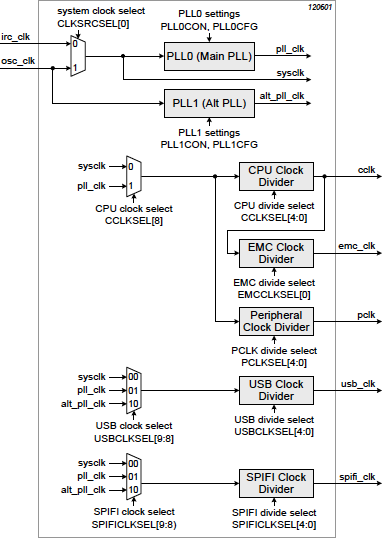
\includegraphics[scale=0.65]{clock-gen}
  \caption{Clock generation}
  \label{fig:clockgeneration}
\end{figure}

\begin{figure}
  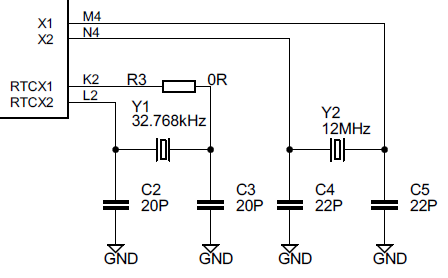
\includegraphics[scale=0.75]{qsb-xtl}
  \caption{Quickstart board Crystal circuit}
  \label{fig:externalxtl}
\end{figure}

Figure \ref{fig:clockgeneration} from \citep[pg. 21]{lpc4088} shows
the various clock generation circuits.   fFigure
\ref{fig:externalxtl} \citep[sheet 2]{quickstart} shows the 
external crystal used as the external oscillator.

The PLL (Phase Locked Loop) is used to boost the input clock signal to
higher frequencies.

The Register \texttt{PLL0CFG} controls the behaviour of the PLL
\citep[sec 3.10.4]{lpc4088}.  
In the startup files \path{system_LPC407x_8x177x_8x.c} and
\path{system_LPC407x_8x177x_8x.h} the values for the PLL and timers
are defined. (see \citep[table 47]{lpc4088} for mapping register
values to $M$ and $P$)
\begin{minted}{C}
#define PLL0CFG_Val           0x00000009
\end{minted}
\begin{table}
  \begin{tabular}{lllrs}
    Quantity & & Source & {Value} \\
    $M$&PLL multiplier&\texttt{PLL0CFG} bits 4:0 & 10 \\
    $P$&PLL divider &\texttt{PLL0CFG} bits 6:5 & 1 \\
    $f_{\mathrm{in}}$&input frequency&external crystal & 12 &
                                                            \mega\hertz \\
  \end{tabular}
  \caption{Values for PLL}
  \label{tab:PLL}
\end{table}
The output frequency of the PLL is given by
\begin{equation}
  f_{\mathrm{out}} = M f_{\mathrm{in}} 
\end{equation}
The current controlled oscillator (internal to the PLL) has a frequency of
\begin{equation}
  f_{\mathrm{CCO}} = 2 M P f_{\mathrm{in}}
\end{equation}
Putting the values into these we get
\begin{table}
  \begin{tabular}{lSs}
    crystal & 12 & \mega\hertz\\
    $f_{\mathrm{in}}$ & 12 & \mega\hertz\\
    $f_{\mathrm{out}}$ & 120 & \mega\hertz\\
    $f_{\mathrm{CCO}}$ & 240 & \mega\hertz
  \end{tabular}
  \caption{Clock and oscilator values}
\end{table}
\subsection{CPU Clock}
The output from the PLL is selected as the CPU clock frequency by the
\texttt{CCLKSEL} register, which also defines the divider value in
bits 4:0 \citep[Table 20, sec3.3.3.2]{lpc4088}.
\begin{minted}{C}
#define CCLKSEL_Val           0x00000101
\end{minted}
The CPU clock divider is 1, so the PLL ouput is used directly as the
clock signal This \SI{120}{\mega\hertz} frequency is made available
from \path{system_LPC407x_8x_177x_8x.c} line 368 as
\texttt{SystemCoreClock}.

\subsection{Peripheral Clock}
The Peripheral Clock signal drives most of the on chip peripherals.
The register \texttt{PCLKSEL} \citep[sectin 3.3.3.5, table
23]{lpc4088} controls the divider value to use
\begin{minted}{C}
#define PCLKSEL_Val           0x00000002
\end{minted}
This gives the divider value as 2.  The peripheral clock is therefore
\SI{60}{\mega\hertz}.  This frequency is made available
from \path{system_LPC407x_8x_177x_8x.c} line 369 as
\texttt{PeripheralClock}.

\section{SysTick}
The SysTick timer is driven by the \SI{120}{\mega\hertz} CPU clock
signal.  The timers  uses a 24bit count down timer, the reset value is
loaded from \texttt{STRELOAD}.
\begin{figure}[h]
  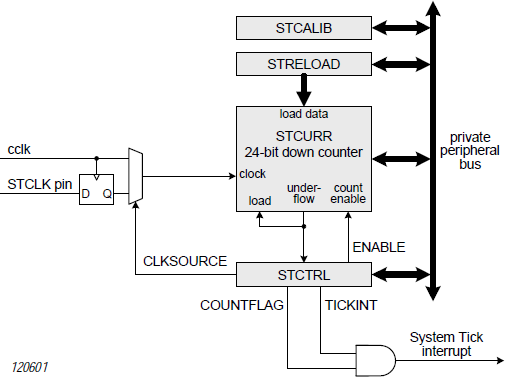
\includegraphics[scale=0.5]{systick}
  \caption{SysTick timer circuit}
  \label{fig:systick}
\end{figure}
Given 24 bits can hold a maximum value of $2^{24}-1$ or \num{16777215}
we get a maximum SysTick period of $2^{24}$ CPU ticks of \SI{0.139810}{s}
\[
  \frac{16777216}{120000000} = 0.139810
\]
Conversely the minimum period is \SI{8}{\nano\second}!
The Cortex M4 User Guide \citep{cortex_m4_user_guide} has a good
description of the SysTick timer operation.

\section{Timer 0/1/2/3}
The timers are covered in \citep[Chapter 24]{lpc4088}.  
Figure \ref{fig:timer} shows the timer circuit.  The peripheral clock
signal drives the timer through the prescale counter.

\subsection{Operation -- prescale and count}
Timer Counter (TC), Prescale Register (PR) and prescale counter
(PC).  The 32 bit TC is incremented every PR+1 cycles of PCLK.
Prescale Register.  When the Prescale Counter (PC) is equal to this
value, the next clock increments the TC and clears the PC.  Prescale
Counter.  The 32 bit PC is a counter which is incremented to the value
stored in PR.  When the value in PR is reached, the TC is incremented
and the PC is cleared.
 
The prescale register therefore is used to scale the CPU clock down to
give the timer clock tick.
\begin{figure}
  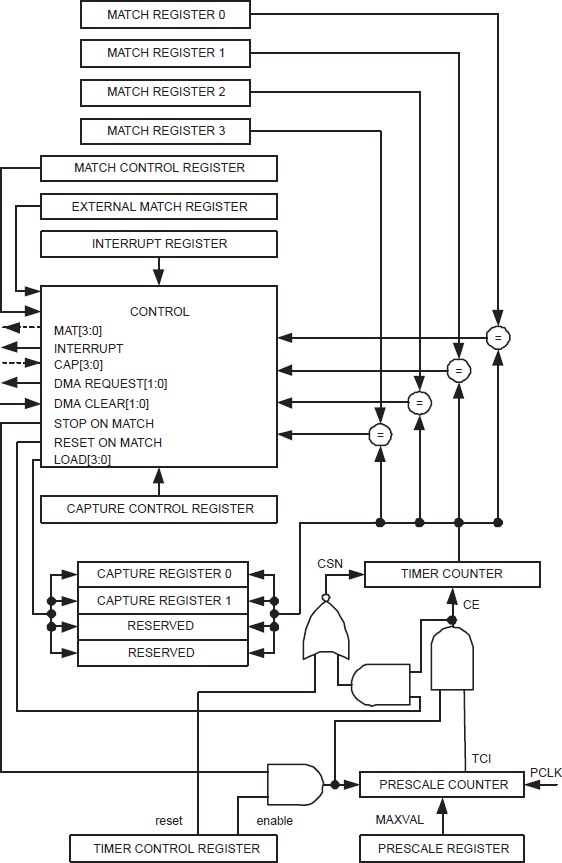
\includegraphics[width=\linewidth]{timercircuit}
  \caption{Timer circuit}
  \label{fig:timer}
\end{figure}

The timer register, counts up on each tick from the prescaler.
When it reaches the value in one of the match registers, the timer
reacts acording to the values in the match control register.

So the relevent relations are shown in table \ref{tab:timer}.
A simple scheme is to set the prescaler to 0 (divide by 1).
The period of the timer, the value to use in the match register is
given by (\texttt{tickHz} is the rate wanted for the timer interrupt).
\begin{minted}{C}
 PeripheralClock / tickHz - 1 
\end{minted}
\begin{table}
  \begin{tabular}{lll}
    Peripheral Clock rate & $f_P$ & \SI{60}{\mega\hertz} \\
    Prescale Register & $\mathrm{PR}$ & \\
    Timer tick rate & $f_T = \frac{f_P}{\mathrm{PR}+1}$ & \\
    Match Register & $\mathrm{MR}$ & \\
    Interupt tick rate & $\frac{f_T}{\mathrm{MR}+1}$ & \\
  \end{tabular}
  \caption{Timer relationships}
  \label{tab:timer}
\end{table}
\label{sec:timer-behavior-end}
The highest rate the timer can run at is one interrupt every tick of
the Peripheral Clock \SI{60}{\mega\hertz} or once every
\SI{16.7}{\nano\second}.  With the prescaler to 0 (divide by 1), the
timer interrupt can occur at a maximum of every $2^{32}$ ticks, or \SI{71.6}{\second}
\[
\frac{2^{32}}{\num{60e6}} = 71.6
\] 
With the prescaler and the match register set to their maximum values,
an interrupt occurs every \SI{307445734561}{\second} or
\num{9749}~years!

\end{document}

% min systick 
% 8ns ~ 
% peripheral clock 60MHz => 16ns (8ns half-life of K meson

%% Local Variables:
%% mode: reftex
%% mode: auto-fill
%% mode: flyspell
%% End: